\documentclass[final]{beamer}
\usepackage{beamerposter} % Use the beamerposter package for laying out the poster
\usetheme{agu2017}
\usepackage[numbers]{natbib}
\usepackage{wrapfig}


%------
% Sizes
\setbeamerfont{title}{size={\fontsize{80}{34}}}
\setbeamerfont{author}{size={\fontsize{50}{40}}}
\setbeamerfont{institute}{size={\fontsize{42}{32}}}
\setbeamerfont{date}{size={\fontsize{38}{32}}}

\setbeamerfont{block title}{size={\fontsize{50}{34}}}
\setbeamerfont{block body}{size={\fontsize{34}{40}}}

\setbeamerfont{block title example}{size={\fontsize{50}{34}}}
\setbeamerfont{block body example}{size={\fontsize{34}{40}}}

\setbeamerfont{block title alerted}{size={\fontsize{50}{34}}}
\setbeamerfont{block alerted body}{size={\fontsize{34}{40}}}
\setbeamerfont{normal text}{size={\fontsize{50}{32}}}
\usebeamerfont{normal text}
%------


%-----------------------------------------------------------
% Define the column widths and overall poster size
% To set effective sepwid, onecolwid and twocolwid values, first choose how many columns you want and how much separation you want between columns
% In this template, the separation width chosen is 0.024 of the paper width and a 4-column layout
% onecolwid should therefore be (1-(# of columns+1)*sepwid)/# of columns e.g. (1-(4+1)*0.024)/4 = 0.22
% Set twocolwid to be (2*onecolwid)+sepwid = 0.464
% Set threecolwid to be (3*onecolwid)+2*sepwid = 0.708
\newlength{\sepwid}
\newlength{\onecolwid}
\newlength{\twocolwid}
\newlength{\threecolwid}
\setlength{\paperwidth}{140cm} % A0 width: 46.8in
\setlength{\paperheight}{100cm} % A0 height: 33.1in
\setlength{\sepwid}{0.01\paperwidth} % Separation width (white space) between columns
\setlength{\onecolwid}{0.309\paperwidth} % Width of one column
\setlength{\twocolwid}{0.65\paperwidth} % Width of two columns
\setlength{\threecolwid}{1\paperwidth} % Width of three columns
\setlength{\topmargin}{-0.5in} % Reduce the top margin size
%-----------------------------------------------------------

\usepackage{graphicx}  % Required for including images
\newcommand{\bsize}{\fontsize{40}{50}\selectfont}
    \usepackage[T1]{fontenc}
    % Nicer default font (+ math font) than Computer Modern for most use cases
    \usepackage{mathpazo}

    % Basic figure setup, for now with no caption control since it's done
    % automatically by Pandoc (which extracts ![](path) syntax from Markdown).
    \usepackage{graphicx}
    % We will generate all images so they have a width \maxwidth. This means
    % that they will get their normal width if they fit onto the page, but
    % are scaled down if they would overflow the margins.
    \makeatletter
    \def\maxwidth{\ifdim\Gin@nat@width>\linewidth\linewidth
    \else\Gin@nat@width\fi}
    \makeatother
%    \let\Oldincludegraphics\includegraphics
    % Set max figure width to be 80% of text width, for now hardcoded.
%    \renewcommand{\includegraphics}[1]{\Oldincludegraphics[width=.8\maxwidth]{#1}}
    % Ensure that by default, figures have no caption (until we provide a
    % proper Figure object with a Caption API and a way to capture that
    % in the conversion process - todo).
    \usepackage{caption}
    \DeclareCaptionLabelFormat{nolabel}{}
    \captionsetup{labelformat=nolabel}

    \usepackage{adjustbox} % Used to constrain images to a maximum size 
    \usepackage{xcolor} % Allow colors to be defined
    \usepackage{enumerate} % Needed for markdown enumerations to work
%    \usepackage{geometry} % Used to adjust the document margins
%    \usepackage{amsmath} % Equations
%    \usepackage{amssymb} % Equations
    \usepackage{textcomp} % defines textquotesingle
    % Hack from http://tex.stackexchange.com/a/47451/13684:
    \AtBeginDocument{%
        \def\PYZsq{\textquotesingle}% Upright quotes in Pygmentized code
    }
    \usepackage{upquote} % Upright quotes for verbatim code
    \usepackage[mathletters]{ucs} % Extended unicode (utf-8) support
    \usepackage[utf8x]{inputenc} % Allow utf-8 characters in the tex document
    \usepackage{fancyvrb} % verbatim replacement that allows latex
    \usepackage{grffile} % extends the file name processing of package graphics 
                         % to support a larger range 
    % The hyperref package gives us a pdf with properly built
    % internal navigation ('pdf bookmarks' for the table of contents,
    % internal cross-reference links, web links for URLs, etc.)
    \usepackage{hyperref}
    \usepackage[normalem]{ulem} % ulem is needed to support strikethroughs (\sout)
    
    
    % Colors for the hyperref package
    \definecolor{urlcolor}{rgb}{0,.145,.698}
    \definecolor{linkcolor}{rgb}{.71,0.21,0.01}
    \definecolor{citecolor}{rgb}{.12,.54,.11}

    % ANSI colors
    \definecolor{ansi-black}{HTML}{3E424D}
    \definecolor{ansi-black-intense}{HTML}{282C36}
    \definecolor{ansi-red}{HTML}{E75C58}
    \definecolor{ansi-red-intense}{HTML}{B22B31}
    \definecolor{ansi-green}{HTML}{00A250}
    \definecolor{ansi-green-intense}{HTML}{007427}
    \definecolor{ansi-yellow}{HTML}{DDB62B}
    \definecolor{ansi-yellow-intense}{HTML}{B27D12}
    \definecolor{ansi-blue}{HTML}{208FFB}
    \definecolor{ansi-blue-intense}{HTML}{0065CA}
    \definecolor{ansi-magenta}{HTML}{D160C4}
    \definecolor{ansi-magenta-intense}{HTML}{A03196}
    \definecolor{ansi-cyan}{HTML}{60C6C8}
    \definecolor{ansi-cyan-intense}{HTML}{258F8F}
    \definecolor{ansi-white}{HTML}{C5C1B4}
    \definecolor{ansi-white-intense}{HTML}{A1A6B2}

    % commands and environments needed by pandoc snippets
    % extracted from the output of `pandoc -s`
%    \providecommand{\tightlist}{%
%      \setlength{\itemsep}{0pt}\setlength{\parskip}{0pt}}
    \DefineVerbatimEnvironment{Highlighting}{Verbatim}{commandchars=\\\{\}}
    % Add ',fontsize=\small' for more characters per line
    \newenvironment{Shaded}{}{}
    \newcommand{\KeywordTok}[1]{\textcolor[rgb]{0.00,0.44,0.13}{\textbf{{#1}}}}
    \newcommand{\DataTypeTok}[1]{\textcolor[rgb]{0.56,0.13,0.00}{{#1}}}
    \newcommand{\DecValTok}[1]{\textcolor[rgb]{0.25,0.63,0.44}{{#1}}}
    \newcommand{\BaseNTok}[1]{\textcolor[rgb]{0.25,0.63,0.44}{{#1}}}
    \newcommand{\FloatTok}[1]{\textcolor[rgb]{0.25,0.63,0.44}{{#1}}}
    \newcommand{\CharTok}[1]{\textcolor[rgb]{0.25,0.44,0.63}{{#1}}}
    \newcommand{\StringTok}[1]{\textcolor[rgb]{0.25,0.44,0.63}{{#1}}}
    \newcommand{\CommentTok}[1]{\textcolor[rgb]{0.38,0.63,0.69}{\textit{{#1}}}}
    \newcommand{\OtherTok}[1]{\textcolor[rgb]{0.00,0.44,0.13}{{#1}}}
    \newcommand{\AlertTok}[1]{\textcolor[rgb]{1.00,0.00,0.00}{\textbf{{#1}}}}
    \newcommand{\FunctionTok}[1]{\textcolor[rgb]{0.02,0.16,0.49}{{#1}}}
    \newcommand{\RegionMarkerTok}[1]{{#1}}
    \newcommand{\ErrorTok}[1]{\textcolor[rgb]{1.00,0.00,0.00}{\textbf{{#1}}}}
    \newcommand{\NormalTok}[1]{{#1}}
    
    % Additional commands for more recent versions of Pandoc
    \newcommand{\ConstantTok}[1]{\textcolor[rgb]{0.53,0.00,0.00}{{#1}}}
    \newcommand{\SpecialCharTok}[1]{\textcolor[rgb]{0.25,0.44,0.63}{{#1}}}
    \newcommand{\VerbatimStringTok}[1]{\textcolor[rgb]{0.25,0.44,0.63}{{#1}}}
    \newcommand{\SpecialStringTok}[1]{\textcolor[rgb]{0.73,0.40,0.53}{{#1}}}
    \newcommand{\ImportTok}[1]{{#1}}
    \newcommand{\DocumentationTok}[1]{\textcolor[rgb]{0.73,0.13,0.13}{\textit{{#1}}}}
    \newcommand{\AnnotationTok}[1]{\textcolor[rgb]{0.38,0.63,0.69}{\textbf{\textit{{#1}}}}}
    \newcommand{\CommentVarTok}[1]{\textcolor[rgb]{0.38,0.63,0.69}{\textbf{\textit{{#1}}}}}
    \newcommand{\VariableTok}[1]{\textcolor[rgb]{0.10,0.09,0.49}{{#1}}}
    \newcommand{\ControlFlowTok}[1]{\textcolor[rgb]{0.00,0.44,0.13}{\textbf{{#1}}}}
    \newcommand{\OperatorTok}[1]{\textcolor[rgb]{0.40,0.40,0.40}{{#1}}}
    \newcommand{\BuiltInTok}[1]{{#1}}
    \newcommand{\ExtensionTok}[1]{{#1}}
    \newcommand{\PreprocessorTok}[1]{\textcolor[rgb]{0.74,0.48,0.00}{{#1}}}
    \newcommand{\AttributeTok}[1]{\textcolor[rgb]{0.49,0.56,0.16}{{#1}}}
    \newcommand{\InformationTok}[1]{\textcolor[rgb]{0.38,0.63,0.69}{\textbf{\textit{{#1}}}}}
    \newcommand{\WarningTok}[1]{\textcolor[rgb]{0.38,0.63,0.69}{\textbf{\textit{{#1}}}}}
    
    
    % Define a nice break command that doesn't care if a line doesn't already
    % exist.
    \def\br{\hspace*{\fill} \\* }
    % Math Jax compatability definitions
    \def\gt{>}
    \def\lt{<}
    % Document parameters
    \title{simple\_case}
    
    
    

    % Pygments definitions
    
\makeatletter
\def\PY@reset{\let\PY@it=\relax \let\PY@bf=\relax%
    \let\PY@ul=\relax \let\PY@tc=\relax%
    \let\PY@bc=\relax \let\PY@ff=\relax}
\def\PY@tok#1{\csname PY@tok@#1\endcsname}
\def\PY@toks#1+{\ifx\relax#1\empty\else%
    \PY@tok{#1}\expandafter\PY@toks\fi}
\def\PY@do#1{\PY@bc{\PY@tc{\PY@ul{%
    \PY@it{\PY@bf{\PY@ff{#1}}}}}}}
\def\PY#1#2{\PY@reset\PY@toks#1+\relax+\PY@do{#2}}

\expandafter\def\csname PY@tok@nt\endcsname{\let\PY@bf=\textbf\def\PY@tc##1{\textcolor[rgb]{0.00,0.50,0.00}{##1}}}
\expandafter\def\csname PY@tok@sr\endcsname{\def\PY@tc##1{\textcolor[rgb]{0.73,0.40,0.53}{##1}}}
\expandafter\def\csname PY@tok@nd\endcsname{\def\PY@tc##1{\textcolor[rgb]{0.67,0.13,1.00}{##1}}}
\expandafter\def\csname PY@tok@ch\endcsname{\let\PY@it=\textit\def\PY@tc##1{\textcolor[rgb]{0.25,0.50,0.50}{##1}}}
\expandafter\def\csname PY@tok@gi\endcsname{\def\PY@tc##1{\textcolor[rgb]{0.00,0.63,0.00}{##1}}}
\expandafter\def\csname PY@tok@kn\endcsname{\let\PY@bf=\textbf\def\PY@tc##1{\textcolor[rgb]{0.00,0.50,0.00}{##1}}}
\expandafter\def\csname PY@tok@mb\endcsname{\def\PY@tc##1{\textcolor[rgb]{0.40,0.40,0.40}{##1}}}
\expandafter\def\csname PY@tok@ge\endcsname{\let\PY@it=\textit}
\expandafter\def\csname PY@tok@nb\endcsname{\def\PY@tc##1{\textcolor[rgb]{0.00,0.50,0.00}{##1}}}
\expandafter\def\csname PY@tok@cm\endcsname{\let\PY@it=\textit\def\PY@tc##1{\textcolor[rgb]{0.25,0.50,0.50}{##1}}}
\expandafter\def\csname PY@tok@k\endcsname{\let\PY@bf=\textbf\def\PY@tc##1{\textcolor[rgb]{0.00,0.50,0.00}{##1}}}
\expandafter\def\csname PY@tok@gd\endcsname{\def\PY@tc##1{\textcolor[rgb]{0.63,0.00,0.00}{##1}}}
\expandafter\def\csname PY@tok@cp\endcsname{\def\PY@tc##1{\textcolor[rgb]{0.74,0.48,0.00}{##1}}}
\expandafter\def\csname PY@tok@o\endcsname{\def\PY@tc##1{\textcolor[rgb]{0.40,0.40,0.40}{##1}}}
\expandafter\def\csname PY@tok@ni\endcsname{\let\PY@bf=\textbf\def\PY@tc##1{\textcolor[rgb]{0.60,0.60,0.60}{##1}}}
\expandafter\def\csname PY@tok@sa\endcsname{\def\PY@tc##1{\textcolor[rgb]{0.73,0.13,0.13}{##1}}}
\expandafter\def\csname PY@tok@bp\endcsname{\def\PY@tc##1{\textcolor[rgb]{0.00,0.50,0.00}{##1}}}
\expandafter\def\csname PY@tok@go\endcsname{\def\PY@tc##1{\textcolor[rgb]{0.53,0.53,0.53}{##1}}}
\expandafter\def\csname PY@tok@il\endcsname{\def\PY@tc##1{\textcolor[rgb]{0.40,0.40,0.40}{##1}}}
\expandafter\def\csname PY@tok@kp\endcsname{\def\PY@tc##1{\textcolor[rgb]{0.00,0.50,0.00}{##1}}}
\expandafter\def\csname PY@tok@ow\endcsname{\let\PY@bf=\textbf\def\PY@tc##1{\textcolor[rgb]{0.67,0.13,1.00}{##1}}}
\expandafter\def\csname PY@tok@gh\endcsname{\let\PY@bf=\textbf\def\PY@tc##1{\textcolor[rgb]{0.00,0.00,0.50}{##1}}}
\expandafter\def\csname PY@tok@gp\endcsname{\let\PY@bf=\textbf\def\PY@tc##1{\textcolor[rgb]{0.00,0.00,0.50}{##1}}}
\expandafter\def\csname PY@tok@c\endcsname{\let\PY@it=\textit\def\PY@tc##1{\textcolor[rgb]{0.25,0.50,0.50}{##1}}}
\expandafter\def\csname PY@tok@si\endcsname{\let\PY@bf=\textbf\def\PY@tc##1{\textcolor[rgb]{0.73,0.40,0.53}{##1}}}
\expandafter\def\csname PY@tok@mf\endcsname{\def\PY@tc##1{\textcolor[rgb]{0.40,0.40,0.40}{##1}}}
\expandafter\def\csname PY@tok@c1\endcsname{\let\PY@it=\textit\def\PY@tc##1{\textcolor[rgb]{0.25,0.50,0.50}{##1}}}
\expandafter\def\csname PY@tok@nn\endcsname{\let\PY@bf=\textbf\def\PY@tc##1{\textcolor[rgb]{0.00,0.00,1.00}{##1}}}
\expandafter\def\csname PY@tok@sh\endcsname{\def\PY@tc##1{\textcolor[rgb]{0.73,0.13,0.13}{##1}}}
\expandafter\def\csname PY@tok@vg\endcsname{\def\PY@tc##1{\textcolor[rgb]{0.10,0.09,0.49}{##1}}}
\expandafter\def\csname PY@tok@no\endcsname{\def\PY@tc##1{\textcolor[rgb]{0.53,0.00,0.00}{##1}}}
\expandafter\def\csname PY@tok@mo\endcsname{\def\PY@tc##1{\textcolor[rgb]{0.40,0.40,0.40}{##1}}}
\expandafter\def\csname PY@tok@err\endcsname{\def\PY@bc##1{\setlength{\fboxsep}{0pt}\fcolorbox[rgb]{1.00,0.00,0.00}{1,1,1}{\strut ##1}}}
\expandafter\def\csname PY@tok@sd\endcsname{\let\PY@it=\textit\def\PY@tc##1{\textcolor[rgb]{0.73,0.13,0.13}{##1}}}
\expandafter\def\csname PY@tok@fm\endcsname{\def\PY@tc##1{\textcolor[rgb]{0.00,0.00,1.00}{##1}}}
\expandafter\def\csname PY@tok@na\endcsname{\def\PY@tc##1{\textcolor[rgb]{0.49,0.56,0.16}{##1}}}
\expandafter\def\csname PY@tok@cpf\endcsname{\let\PY@it=\textit\def\PY@tc##1{\textcolor[rgb]{0.25,0.50,0.50}{##1}}}
\expandafter\def\csname PY@tok@gt\endcsname{\def\PY@tc##1{\textcolor[rgb]{0.00,0.27,0.87}{##1}}}
\expandafter\def\csname PY@tok@nf\endcsname{\def\PY@tc##1{\textcolor[rgb]{0.00,0.00,1.00}{##1}}}
\expandafter\def\csname PY@tok@nv\endcsname{\def\PY@tc##1{\textcolor[rgb]{0.10,0.09,0.49}{##1}}}
\expandafter\def\csname PY@tok@sc\endcsname{\def\PY@tc##1{\textcolor[rgb]{0.73,0.13,0.13}{##1}}}
\expandafter\def\csname PY@tok@dl\endcsname{\def\PY@tc##1{\textcolor[rgb]{0.73,0.13,0.13}{##1}}}
\expandafter\def\csname PY@tok@s\endcsname{\def\PY@tc##1{\textcolor[rgb]{0.73,0.13,0.13}{##1}}}
\expandafter\def\csname PY@tok@m\endcsname{\def\PY@tc##1{\textcolor[rgb]{0.40,0.40,0.40}{##1}}}
\expandafter\def\csname PY@tok@kt\endcsname{\def\PY@tc##1{\textcolor[rgb]{0.69,0.00,0.25}{##1}}}
\expandafter\def\csname PY@tok@mh\endcsname{\def\PY@tc##1{\textcolor[rgb]{0.40,0.40,0.40}{##1}}}
\expandafter\def\csname PY@tok@ss\endcsname{\def\PY@tc##1{\textcolor[rgb]{0.10,0.09,0.49}{##1}}}
\expandafter\def\csname PY@tok@gu\endcsname{\let\PY@bf=\textbf\def\PY@tc##1{\textcolor[rgb]{0.50,0.00,0.50}{##1}}}
\expandafter\def\csname PY@tok@mi\endcsname{\def\PY@tc##1{\textcolor[rgb]{0.40,0.40,0.40}{##1}}}
\expandafter\def\csname PY@tok@s2\endcsname{\def\PY@tc##1{\textcolor[rgb]{0.73,0.13,0.13}{##1}}}
\expandafter\def\csname PY@tok@w\endcsname{\def\PY@tc##1{\textcolor[rgb]{0.73,0.73,0.73}{##1}}}
\expandafter\def\csname PY@tok@sx\endcsname{\def\PY@tc##1{\textcolor[rgb]{0.00,0.50,0.00}{##1}}}
\expandafter\def\csname PY@tok@gs\endcsname{\let\PY@bf=\textbf}
\expandafter\def\csname PY@tok@vc\endcsname{\def\PY@tc##1{\textcolor[rgb]{0.10,0.09,0.49}{##1}}}
\expandafter\def\csname PY@tok@cs\endcsname{\let\PY@it=\textit\def\PY@tc##1{\textcolor[rgb]{0.25,0.50,0.50}{##1}}}
\expandafter\def\csname PY@tok@vm\endcsname{\def\PY@tc##1{\textcolor[rgb]{0.10,0.09,0.49}{##1}}}
\expandafter\def\csname PY@tok@kc\endcsname{\let\PY@bf=\textbf\def\PY@tc##1{\textcolor[rgb]{0.00,0.50,0.00}{##1}}}
\expandafter\def\csname PY@tok@nl\endcsname{\def\PY@tc##1{\textcolor[rgb]{0.63,0.63,0.00}{##1}}}
\expandafter\def\csname PY@tok@gr\endcsname{\def\PY@tc##1{\textcolor[rgb]{1.00,0.00,0.00}{##1}}}
\expandafter\def\csname PY@tok@sb\endcsname{\def\PY@tc##1{\textcolor[rgb]{0.73,0.13,0.13}{##1}}}
\expandafter\def\csname PY@tok@kd\endcsname{\let\PY@bf=\textbf\def\PY@tc##1{\textcolor[rgb]{0.00,0.50,0.00}{##1}}}
\expandafter\def\csname PY@tok@nc\endcsname{\let\PY@bf=\textbf\def\PY@tc##1{\textcolor[rgb]{0.00,0.00,1.00}{##1}}}
\expandafter\def\csname PY@tok@vi\endcsname{\def\PY@tc##1{\textcolor[rgb]{0.10,0.09,0.49}{##1}}}
\expandafter\def\csname PY@tok@ne\endcsname{\let\PY@bf=\textbf\def\PY@tc##1{\textcolor[rgb]{0.82,0.25,0.23}{##1}}}
\expandafter\def\csname PY@tok@kr\endcsname{\let\PY@bf=\textbf\def\PY@tc##1{\textcolor[rgb]{0.00,0.50,0.00}{##1}}}
\expandafter\def\csname PY@tok@se\endcsname{\let\PY@bf=\textbf\def\PY@tc##1{\textcolor[rgb]{0.73,0.40,0.13}{##1}}}
\expandafter\def\csname PY@tok@s1\endcsname{\def\PY@tc##1{\textcolor[rgb]{0.73,0.13,0.13}{##1}}}

\def\PYZbs{\char`\\}
\def\PYZus{\char`\_}
\def\PYZob{\char`\{}
\def\PYZcb{\char`\}}
\def\PYZca{\char`\^}
\def\PYZam{\char`\&}
\def\PYZlt{\char`\<}
\def\PYZgt{\char`\>}
\def\PYZsh{\char`\#}
\def\PYZpc{\char`\%}
\def\PYZdl{\char`\$}
\def\PYZhy{\char`\-}
\def\PYZsq{\char`\'}
\def\PYZdq{\char`\"}
\def\PYZti{\char`\~}
% for compatibility with earlier versions
\def\PYZat{@}
\def\PYZlb{[}
\def\PYZrb{]}
\makeatother


    % Exact colors from NB
    \definecolor{incolor}{rgb}{0.0, 0.0, 0.5}
    \definecolor{outcolor}{rgb}{0.545, 0.0, 0.0}



    
    % Prevent overflowing lines due to hard-to-break entities
    \sloppy 
    % Setup hyperref package
    \hypersetup{
      breaklinks=true,  % so long urls are correctly broken across lines
      colorlinks=true,
      urlcolor=urlcolor,
      linkcolor=linkcolor,
      citecolor=citecolor,
      }




%----------------------------------------------------------------------------------------
%   TITLE SECTION 
\title{{\fontsize{180}{50}\selectfont Pymicra:}\newline A Python tool for Micrometerological Analyses} % Poster title

\author{
\newauthor{Tomás L. Chor\inst{1}}{tomaschor@ucla.edu}\and\newauthor{Nelson L. Dias\inst{2}}{nldias@ufpr.br}
}
\institute{
\inst{1} University of California, Los Angeles, Department of Atmospheric and Oceanic Sciences \and
\inst{2} Federal University of Paraná, Department of Environmental Engineering }
\date{}
%----------------------------------------------------------------------------------------


%----------------------------------------------------------------------------------------
\begin{document}

\begin{frame}[t] % The whole poster is enclosed in one beamer frame

\begin{columns}[t] % The whole poster consists of three major columns, the second of which is split into two columns twice - the [t] option aligns each column's content to the top

\begin{column}{2\sepwid}\end{column} % Empty spacer column


%--------------------
% FIRST COLUMN
%--------------------
\begin{column}{\onecolwid} % The first column

%----------------------------------------------------------------------------------------
%   SUMMARY AND INTRODUCTION
%----------------------------------------------------------------------------------------

\begin{alertblock}{Summary}
\bsize
Pymicra is a Python package that is designed to make micrometeorological data
processing significantly more efficient.

\vspace{.5cm}
It was written with the goal of becoming a community-driven software that is a
full-blown micrometeorology package, not an just eddy-covariance one. It was
designed to make research more efficient and to make sharing code easier and it
was motivated by many examples of similar initiatives that thrived: Obspy for
seismologists \citep{obspy}, Astropy for astrophysicists \citep{astropy}, Sunpy
for solar physicists \citep{sunpy}, Metpy for weather scientists \citep{metpy},
etc.

Here are a few characteristics that make Pymicra a good candidate to be
community-driven:
\begin{itemize}
\item Open-source
\item Code written with Pymicra is very readable and intuitive
\item Visualization of data is extremely easy
\item Easy to develop upon (because of well-documented Python code)
\item Based on well-known mature Python packages
\end{itemize}

\vspace{.5cm}
Pymicra's philosophy is not to "reinvent the wheel". There are already
several open-source packages that process, organize and manipulate data very
efficiently, so the goal was simply to put them together is a way specifically
designed to the micrometeorological community.

\end{alertblock}

%----------------------------------------------------------------------------------------
%   CODE SNIPETS
%----------------------------------------------------------------------------------------
\begin{exampleblock}{Quality control example}
    \begin{Verbatim}[commandchars=\\\{\}]
{\color{incolor}In [{\color{incolor}1}]:} \PY{n}{fnames} \PY{o}{=} \PY{n+nb}{sorted}\PY{p}{(}\PY{n}{glob}\PY{p}{(}\PY{l+s+s1}{\PYZsq{}}\PY{l+s+s1}{mydata/*.out}\PY{l+s+s1}{\PYZsq{}}\PY{p}{)}\PY{p}{)}
        \PY{c+c1}{\PYZsh{} Prints reports on screen and writes further info to file}
        \PY{n}{pymicra}\PY{o}{.}\PY{n}{util}\PY{o}{.}\PY{n}{qc\PYZus{}replace}\PY{p}{(}\PY{n}{fnames}\PY{p}{,} \PY{n}{fconfig}\PY{p}{,}
            \PY{n}{file\PYZus{}lines}\PY{o}{=}\PY{l+m+mi}{36000}\PY{p}{,}
            \PY{n}{lower\PYZus{}limits}\PY{o}{=}\PY{n+nb}{dict}\PY{p}{(}\PY{n}{theta\PYZus{}v}\PY{o}{=}\PY{l+m+mi}{10}\PY{p}{,} \PY{n}{mrho\PYZus{}h2o}\PY{o}{=}\PY{l+m+mi}{0}\PY{p}{,} \PY{n}{mrho\PYZus{}co2}\PY{o}{=}\PY{l+m+mi}{0}\PY{p}{)}\PY{p}{,}
            \PY{n}{upper\PYZus{}limits}\PY{o}{=}\PY{n+nb}{dict}\PY{p}{(}\PY{n}{theta\PYZus{}v}\PY{o}{=}\PY{l+m+mi}{45}\PY{p}{)}\PY{p}{,}
            \PY{n}{spikes\PYZus{}test}\PY{o}{=}\PY{k+kc}{True}\PY{p}{,}
            \PY{n}{max\PYZus{}replacement\PYZus{}count}\PY{o}{=}\PY{l+m+mi}{360}\PY{p}{,}
            \PY{n}{chunk\PYZus{}size}\PY{o}{=}\PY{l+m+mi}{1200}\PY{p}{,}
            \PY{n}{outdir}\PY{o}{=}\PY{l+s+s1}{\PYZsq{}}\PY{l+s+s1}{out1}\PY{l+s+s1}{\PYZsq{}}\PY{p}{,}
            \PY{n}{replaced\PYZus{}report}\PY{o}{=}\PY{l+s+s1}{\PYZsq{}}\PY{l+s+s1}{rrep.txt}\PY{l+s+s1}{\PYZsq{}}\PY{p}{)}
        
        \PY{n}{fnames2} \PY{o}{=} \PY{n+nb}{sorted}\PY{p}{(}\PY{n}{glob}\PY{p}{(}\PY{l+s+s1}{\PYZsq{}}\PY{l+s+s1}{out1/*.out}\PY{l+s+s1}{\PYZsq{}}\PY{p}{)}\PY{p}{)}
        \PY{c+c1}{\PYZsh{} Prints reports on screen and writes further info to file}
        \PY{n}{pymicra}\PY{o}{.}\PY{n}{util}\PY{o}{.}\PY{n}{qc\PYZus{}discard}\PY{p}{(}\PY{n}{fnames2}\PY{p}{,} \PY{n}{fconfig}\PY{p}{,}
            \PY{n}{std\PYZus{}limits} \PY{o}{=} \PY{n+nb}{dict}\PY{p}{(}\PY{n}{u}\PY{o}{=}\PY{l+m+mf}{0.03}\PY{p}{,} \PY{n}{v}\PY{o}{=}\PY{l+m+mf}{0.03}\PY{p}{,} \PY{n}{w}\PY{o}{=}\PY{l+m+mf}{0.01}\PY{p}{,} \PY{n}{theta\PYZus{}v}\PY{o}{=}\PY{l+m+mf}{0.02}\PY{p}{)}\PY{p}{,}
            \PY{n}{dif\PYZus{}limits} \PY{o}{=} \PY{n+nb}{dict}\PY{p}{(}\PY{n}{u}\PY{o}{=}\PY{l+m+mf}{4.0}\PY{p}{,} \PY{n}{v}\PY{o}{=}\PY{l+m+mf}{4.0}\PY{p}{,} \PY{n}{w}\PY{o}{=}\PY{l+m+mf}{1.0}\PY{p}{,} \PY{n}{theta\PYZus{}v}\PY{o}{=}\PY{l+m+mf}{2.0}\PY{p}{)}\PY{p}{,}
            \PY{n}{chunk\PYZus{}size}\PY{o}{=}\PY{l+m+mi}{1200}\PY{p}{,}
            \PY{n}{outdir}\PY{o}{=}\PY{l+s+s1}{\PYZsq{}}\PY{l+s+s1}{out2}\PY{l+s+s1}{\PYZsq{}}\PY{p}{,}
            \PY{n}{summary\PYZus{}file}\PY{o}{=}\PY{l+s+s1}{\PYZsq{}}\PY{l+s+s1}{discard\PYZus{}summary.csv}\PY{l+s+s1}{\PYZsq{}}\PY{p}{,}
            \PY{n}{full\PYZus{}report}\PY{o}{=}\PY{l+s+s1}{\PYZsq{}}\PY{l+s+s1}{frep.txt}\PY{l+s+s1}{\PYZsq{}}\PY{p}{)}
\end{Verbatim}
\end{exampleblock}

\begin{exampleblock}{Pre-processing and calculation of fluxes example}
    \begin{Verbatim}[commandchars=\\\{\}]
{\color{incolor}In [{\color{incolor}2}]:} \PY{n}{fconfig} \PY{o}{=} \PY{n}{pymicra}\PY{o}{.}\PY{n}{fileConfig}\PY{p}{(}\PY{l+s+s1}{\PYZsq{}}\PY{l+s+s1}{tij\PYZus{}pr.config}\PY{l+s+s1}{\PYZsq{}}\PY{p}{)}
        \PY{n}{sconfig} \PY{o}{=} \PY{n}{pymicra}\PY{o}{.}\PY{n}{siteConfig}\PY{p}{(}\PY{l+s+s1}{\PYZsq{}}\PY{l+s+s1}{tij\PYZus{}pr.site}\PY{l+s+s1}{\PYZsq{}}\PY{p}{)}
        \PY{n}{fname} \PY{o}{=} \PY{l+s+s1}{\PYZsq{}}\PY{l+s+s1}{out2/20110224\PYZhy{}1340.out}\PY{l+s+s1}{\PYZsq{}}
        
        \PY{n}{data}\PY{p}{,} \PY{n}{units} \PY{o}{=} \PY{n}{pymicra}\PY{o}{.}\PY{n}{timeSeries}\PY{p}{(}\PY{n}{fname}\PY{p}{,} \PY{n}{fconfig}\PY{p}{,}
                                         \PY{n}{parse\PYZus{}dates}\PY{o}{=}\PY{k+kc}{False}\PY{p}{)}
        \PY{c+c1}{\PYZsh{} Prints reports showing which calculations are being done}
        \PY{n}{data} \PY{o}{=} \PY{n}{pymicra}\PY{o}{.}\PY{n}{micro}\PY{o}{.}\PY{n}{preProcess}\PY{p}{(}\PY{n}{data}\PY{p}{,} \PY{n}{units}\PY{p}{,} \PY{n}{solutes}\PY{o}{=}\PY{p}{[}\PY{l+s+s1}{\PYZsq{}}\PY{l+s+s1}{co2}\PY{l+s+s1}{\PYZsq{}}\PY{p}{]}\PY{p}{)}
        \PY{n}{fulldata} \PY{o}{=} \PY{n}{data}\PY{o}{.}\PY{n}{detrend}\PY{p}{(}\PY{n}{units}\PY{o}{=}\PY{n}{units}\PY{p}{,} \PY{n}{ignore}\PY{o}{=}\PY{p}{[}\PY{l+s+s1}{\PYZsq{}}\PY{l+s+s1}{p}\PY{l+s+s1}{\PYZsq{}}\PY{p}{]}\PY{p}{,}
                                \PY{n}{join\PYZus{}data}\PY{o}{=}\PY{k+kc}{True}\PY{p}{)}
        \PY{c+c1}{\PYZsh{} Prints reports showing which calculations are being done}
        \PY{n}{results} \PY{o}{=} \PY{n}{pymicra}\PY{o}{.}\PY{n}{micro}\PY{o}{.}\PY{n}{eddyCovariance}\PY{p}{(}\PY{n}{fulldata}\PY{p}{,} \PY{n}{units}\PY{p}{,} 
                     \PY{n}{site\PYZus{}config}\PY{o}{=}\PY{n}{sconfig}\PY{p}{,} \PY{n}{wpl}\PY{o}{=}\PY{k+kc}{True}\PY{p}{,} \PY{n}{solutes}\PY{o}{=}\PY{p}{[}\PY{l+s+s1}{\PYZsq{}}\PY{l+s+s1}{co2}\PY{l+s+s1}{\PYZsq{}}\PY{p}{]}\PY{p}{)}
\end{Verbatim}


\end{exampleblock}

    


\end{column} % End of the first column






%--------------------
% SECOND COLUMN
%--------------------
\begin{column}{\sepwid}\end{column} % Empty spacer column
\begin{column}{\onecolwid} % Begin a column which is two columns wide (column 2)
\maketitle
\vspace{-2cm}

\begin{exampleblock}{Visualization example}
    \begin{Verbatim}[commandchars=\\\{\}]
{\color{incolor}In [{\color{incolor}3}]:} \PY{n}{data}\PY{p}{[}\PY{p}{[}\PY{l+s+s1}{\PYZsq{}}\PY{l+s+s1}{u}\PY{l+s+s1}{\PYZsq{}}\PY{p}{,} \PY{l+s+s1}{\PYZsq{}}\PY{l+s+s1}{v}\PY{l+s+s1}{\PYZsq{}}\PY{p}{,} \PY{l+s+s1}{\PYZsq{}}\PY{l+s+s1}{w}\PY{l+s+s1}{\PYZsq{}}\PY{p}{]}\PY{p}{]}\PY{o}{.}\PY{n}{plot}\PY{p}{(}\PY{n}{grid}\PY{o}{=}\PY{k+kc}{True}\PY{p}{)}
        \PY{n}{plt}\PY{o}{.}\PY{n}{show}\PY{p}{(}\PY{p}{)}
\end{Verbatim}


    \begin{center}
    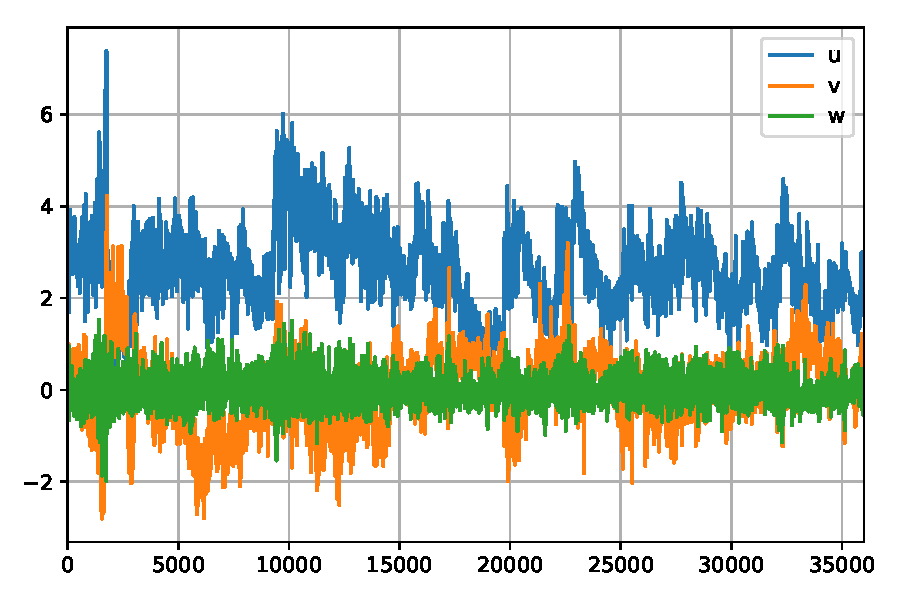
\includegraphics[width=.83\columnwidth]{pprog/uvw.pdf}
    \end{center}
    { \hspace*{\fill} \\}
    
    \begin{Verbatim}[commandchars=\\\{\}]
{\color{incolor}In [{\color{incolor}4}]:} \PY{n}{uw\PYZus{}spectra} \PY{o}{=} \PY{n}{pymicra}\PY{o}{.}\PY{n}{spectra}\PY{p}{(}\PY{n}{fulldata}\PY{p}{[}\PY{p}{[}\PY{l+s+s2}{\PYZdq{}}\PY{l+s+s2}{u}\PY{l+s+s2}{\PYZsq{}}\PY{l+s+s2}{\PYZdq{}}\PY{p}{,} \PY{l+s+s2}{\PYZdq{}}\PY{l+s+s2}{w}\PY{l+s+s2}{\PYZsq{}}\PY{l+s+s2}{\PYZdq{}}\PY{p}{]}\PY{p}{]}\PY{p}{,} 
                                     \PY{n}{frequency}\PY{o}{=}\PY{l+m+mi}{20}\PY{p}{,}
                                     \PY{n}{anti\PYZus{}aliasing}\PY{o}{=}\PY{k+kc}{True}\PY{p}{)}
        axis \PY{o}{=} \PY{n}{uw\PYZus{}spectra}\PY{o}{.}\PY{n}{binned}\PY{p}{(}\PY{n}{bins\PYZus{}number}\PY{o}{=}\PY{l+m+mi}{100}\PY{p}{)}\PY{o}{.}\PY{n}{plot}\PY{p}{(}\PY{n}{loglog}\PY{o}{=}\PY{k+kc}{True}\PY{p}{,}
                                     \PY{n}{grid}\PY{o}{=}\PY{k+kc}{True}\PY{p}{)}
        axis.plot(uw_spectra.index, \PY{l+m+mi}{1e-1}*uw_spectra.index**(\PY{l+m+mi}{-5/3}),
                                     label=\PY{l+s+s2}{'-5/3'})
        \PY{n}{axis}\PY{o}{.}\PY{n}{legend}\PY{p}{(}\PY{p}{)}; \PY{n}{plt}\PY{o}{.}\PY{n}{show}\PY{p}{(}\PY{p}{)}
\end{Verbatim}


    \begin{center}
%    \adjustimage{max size={0.9\linewidth}{0.9\paperheight}}{pprog/all_poster_files/all_poster_8_0.png}
    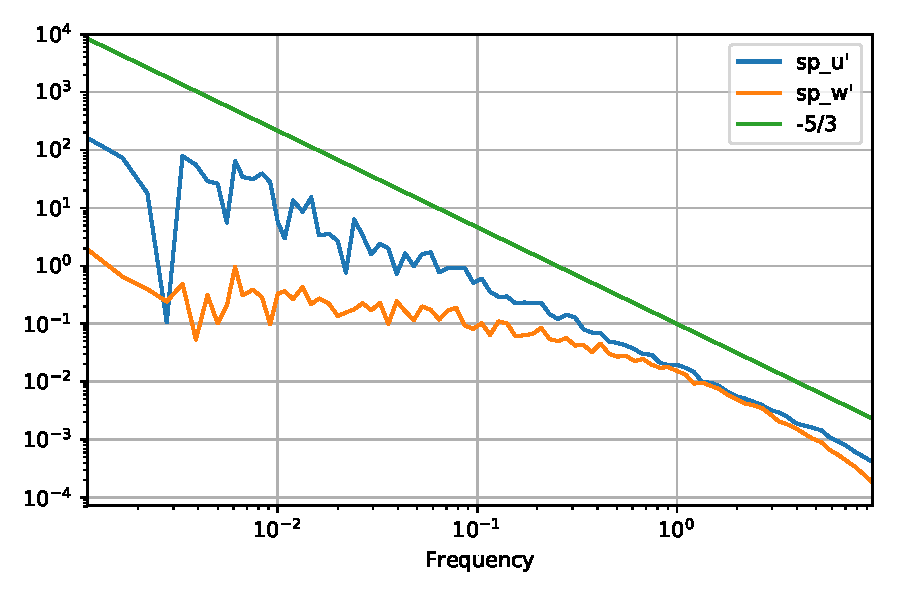
\includegraphics[width=.83\columnwidth]{pprog/spec.pdf}
    \end{center}
    %{ \hspace*{\fill} \\}
    \end{exampleblock}

    



\end{column} % End of the second column





%--------------------
% THIRD COLUMN
%--------------------
\begin{column}{\sepwid}\end{column} % Empty spacer column
\begin{column}{\onecolwid} % The third column

\begin{center}
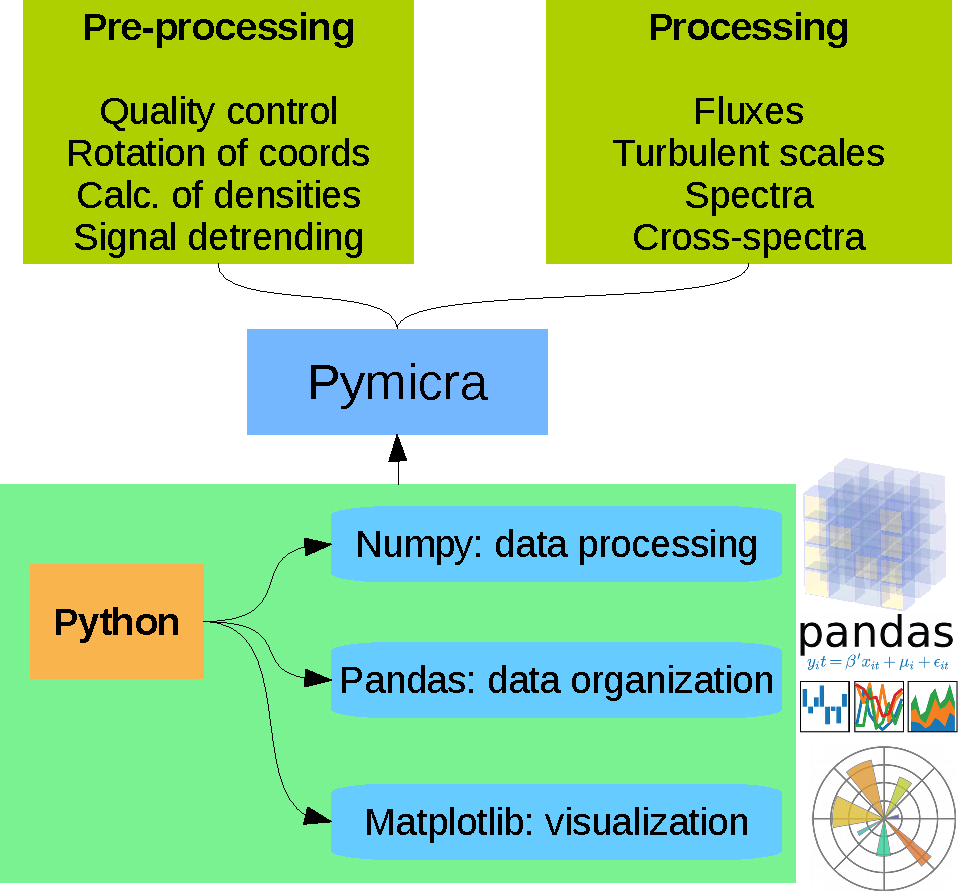
\includegraphics[width=.94\columnwidth]{figs/FC2.pdf}
\end{center}

\setbeamercolor{block alerted title}{fg=black,bg=norange} % Change the alert block title colors
\setbeamercolor{block alerted body}{fg=black,bg=white} % Change the alert block body colors




\begin{alertblock}{Why Pymicra instead of writing my own code?}
\bsize
There are many advantages in migrating to a community package such as Pymicra
aims to be, both community-wise and for the individual: 
\begin{itemize}
\item Package becomes very reliable (more people are constantly checking for
bugs and improving)
\item The amount of code to process the data is significantly smaller (thus faster
to write)
\item Sharing your code and understanding other people's is easier
\end{itemize}

\vspace{1cm}

\begin{minipage}[]{.74\columnwidth}
\begin{itemize}
\item Code adaptability (no need to keep writing \emph{ad hoc} code for each dataset)
\item Flexibility (you can easily use Pymicra to do basic processing and link it
to other tools for more specific things)
\end{itemize}
\end{minipage}
\begin{minipage}[]{.25\columnwidth}
\begin{flushright}
Pymicra's docs $\downarrow$
\includegraphics[width=.75\columnwidth]{main_qrcode.eps}
\end{flushright}
\end{minipage}
\end{alertblock}


\begin{alertblock}{How to contribute}
\bsize

The code is hosted on Github and any person can fork, develop functionality into
it and request a merge back. 

\begin{minipage}[]{.74\columnwidth}
Bug reports, suggestions and documentation
improvements are also very welcome via Github issues or via email.

\vspace{.3cm}
Scan the QR code for more information on contributing.
%$\rightarrow$

\end{minipage}
\begin{minipage}[]{.25\columnwidth}
\begin{flushright}
\includegraphics[width=.75\columnwidth]{contr_qrcode.eps}
\end{flushright}
\end{minipage}
\end{alertblock}

%\vspace{1cm}

\begin{block}{}
\bibliography{refs/posterrefs2.bib}
\bibliographystyle{abbrvnat}
\end{block}
%----------------------------------------------------------------------------------------

\end{column} % End of the third column

\end{columns} % End of all the columns in the poster

\end{frame} % End of the enclosing frame

\end{document}

              

